% UQ Gemini theme
% See: https://github.com/alfurka/gemini-uq
% Forked from
% https://rev.cs.uchicago.edu/k4rtik/gemini-uccs
% which is forked from
% https://github.com/anishathalye/gemini


\documentclass[final]{beamer}

% ====================
% Packages
% ====================

\usepackage[T1]{fontenc}
\usepackage{xcolor}
\usepackage{lmodern}
\usepackage[size=custom,width=100,height=75,scale=1.0]{beamerposter}
\usetheme{gemini}
\usecolortheme{gemini}
\usepackage{graphicx}
\usepackage{booktabs}
\usepackage{tikz}
\usepackage{pgfplots}
\pgfplotsset{compat=1.17}

% ====================
% Lengths
% ====================

% If you have N columns, choose \sepwidth and \colwidth such that
% (N+1)*\sepwidth + N*\colwidth = \paperwidth
\newlength{\sepwidth}
\newlength{\colwidth}
\setlength{\sepwidth}{0.025\paperwidth}
\setlength{\colwidth}{0.3\paperwidth}

\newcommand{\separatorcolumn}{\begin{column}{\sepwidth}\end{column}}


% ====================
% Title
% ====================

\title{Running a Carpentries Workshop without the Internet}

\author{Jannetta S. Steyn \inst{1} \and Colin Sauze \inst{2} \and Abhishek Dasgupta \inst{3}}

\institute[shortinst]{\inst{1} Newcastle University \samelineand \inst{2}National Oceanography Centre \samelineand \inst{3} University of Oxford} 

% ====================
% Footer (optional)
% ====================

\footercontent{
	\href{https://carpentriesoffline.org}{https://carpentriesoffline.org} \hfill
	RSECon 2023 - Swansea \hfill
	\href{mailto:jannetta.steyn@newcastle.ac.uk}{jannetta.steyn@newcastle.ac.uk}
}
% (can be left out to remove footer)

% ====================
% Logo (optional)
% ====================

% use this to include logos on the left and/or right side of the header:
% \logoright{\includegraphics[height=7cm]{logo1.pdf}}
% \logoleft{\includegraphics[height=7cm]{logo2.pdf}}

% ====================
% Body
% ====================

\begin{document}
	\addtobeamertemplate{headline}{}
	{
		\begin{tikzpicture}[remember picture,overlay]
			\node [anchor=north west, inner sep=3cm] at ([xshift=-0.5cm,yshift=0.5cm]current page.north west)
			{\includegraphics[height=4.5cm]{logos/OFFLINE.png}}; % also try shield-white.eps
			\node [anchor=north east, inner sep=3cm] at ([xshift=0.0cm,yshift=2.5cm]current page.north east)
			{\includegraphics[height=8.0cm]{logos/qr.png}};
		\end{tikzpicture}
	}
	
	\begin{frame}[t]
		\begin{block}{\large Abstract}	

			CarpentriesOffline (https://carpentriesoffline.org) is an out of the box solution for running a Carpentries workshop from a single device such as a Raspberry Pi, old laptop or even a dedicated server. It is intended for use in environments where there is limited or no internet access. Everything needed to run the workshop including course notes, data files, software downloads, a Git server, etherpad and a JupyterHub server are provided by the CarpentriesOffline system. It can also provide a backup environment for those with better connectivity in the event of the Carpentries website, etherpad, GitHub etc suffering an outage.
		\end{block}
	
		\begin{columns}[t]
			\separatorcolumn
			
			
			\begin{column}{\colwidth}
				
				\begin{block}{Raspberry Pi Solution}
					\begin{center}
						\begin{figure}
							\includegraphics[width=0.6\columnwidth]{logos/CarpentriesOfflinePhoto.png}
							\caption{A Raspberry Pi Zero running CarpentriesOffline on RPi OS and powered with a USB Power Bank - tested at RSECon2022}
						\end{figure}
					\end{center}

					
				\end{block}
				
				\begin{alertblock}{A highlighted block}
					
					This block catches your eye, so \textbf{important stuff} should probably go
					here.
					
					Curabitur eu libero vehicula, cursus est fringilla, luctus est. Morbi
					consectetur mauris quam, at finibus elit auctor ac. Aliquam erat volutpat.
					Aenean at nisl ut ex ullamcorper eleifend et eu augue. Aenean quis velit
					tristique odio convallis ultrices a ac odio.
					
					\begin{itemize}
						\item \textbf{Fusce dapibus tellus} vel tellus semper finibus. In
						consequat, nibh sed mattis luctus, augue diam fermentum lectus.
						\item \textbf{In euismod erat metus} non ex. Vestibulum luctus augue in
						mi condimentum, at sollicitudin lorem viverra.
						\item \textbf{Suspendisse vulputate} mauris vel placerat consectetur.
						Mauris semper, purus ac hendrerit molestie, elit mi dignissim odio, in
						suscipit felis sapien vel ex.
					\end{itemize}
					
					Aenean tincidunt risus eros, at gravida lorem sagittis vel. Vestibulum ante
					ipsum primis in faucibus orci luctus et ultrices posuere cubilia Curae.
					
				\end{alertblock}
				
			\end{column}
			
			\separatorcolumn
			
			\begin{column}{\colwidth}
				
				\begin{block}{FlashDrive Solution}
					\begin{figure}
						\begin{center}
							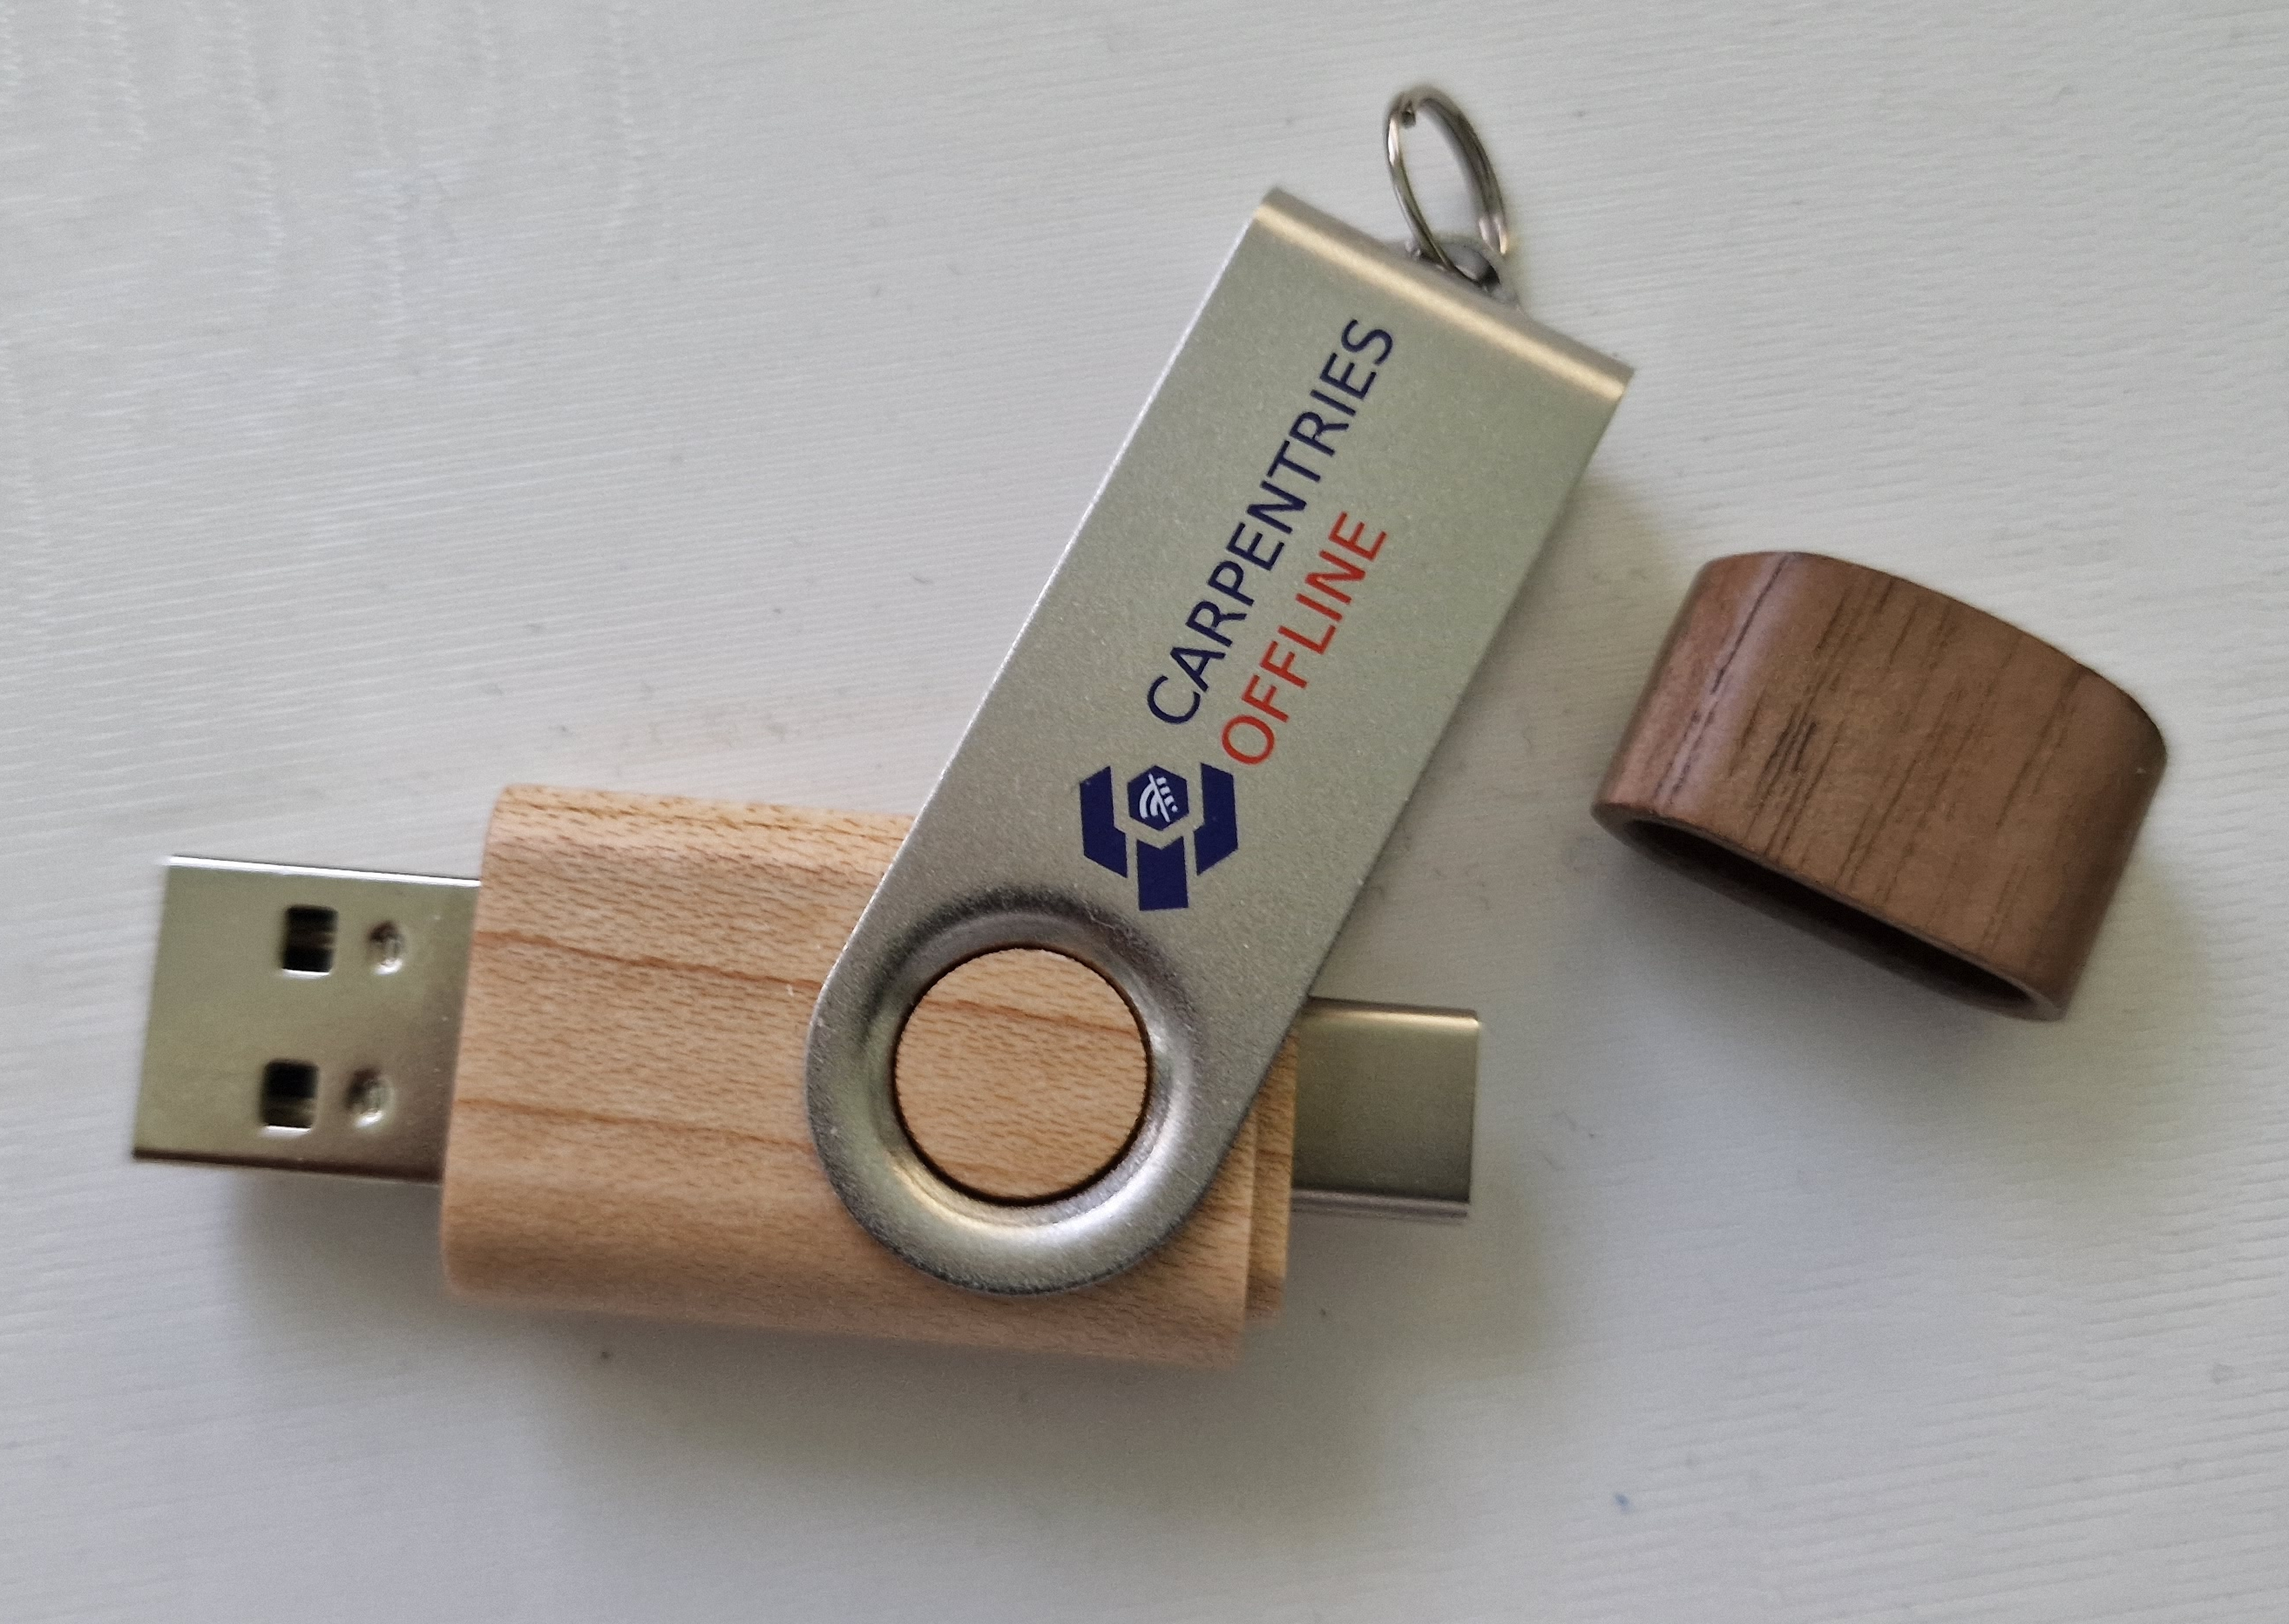
\includegraphics[width=0.6\columnwidth]{logos/FlashDrive.png}
							\caption{A bootable flashdrive with Debian based Slax Linux and everything needed to turn a laptop into an access point and a web server}
						\end{center}
					\end{figure}
				\end{block}
				\begin{alertblock}{A highlighted block}
				
					Some text
				
				\end{alertblock}
				\begin{block}
	afdfadsfasdfasd
	asdfasdfasdfds
	
	
					Vivamus congue volutpat elit non semper. Praesent molestie nec erat ac
					interdum. In quis suscipit erat. \textbf{Phasellus mauris felis, molestie
						ac pharetra quis}, tempus nec ante. Donec finibus ante vel purus mollis
					fermentum. Sed felis mi, pharetra eget nibh a, feugiat eleifend dolor. Nam
					mollis condimentum purus quis sodales. Nullam eu felis eu nulla eleifend
					bibendum nec eu lorem. Vivamus felis velit, volutpat ut facilisis ac,
					commodo in metus.
					
					\begin{enumerate}
						\item \textbf{Morbi mauris purus}, egestas at vehicula et, convallis
						accumsan orci. Orci varius natoque penatibus et magnis dis parturient
						montes, nascetur ridiculus mus.
						\item \textbf{Cras vehicula blandit urna ut maximus}. Aliquam blandit nec
						massa ac sollicitudin. Curabitur cursus, metus nec imperdiet bibendum,
						velit lectus faucibus dolor, quis gravida metus mauris gravida turpis.
						\item \textbf{Vestibulum et massa diam}. Phasellus fermentum augue non
						nulla accumsan, non rhoncus lectus condimentum.
					\end{enumerate}
					
				\end{block}		
			\end{column}
			
			\separatorcolumn
			
			\begin{column}{\colwidth}
				
				\begin{block}{The miniHPC }

					\begin{figure}
						\begin{center}
							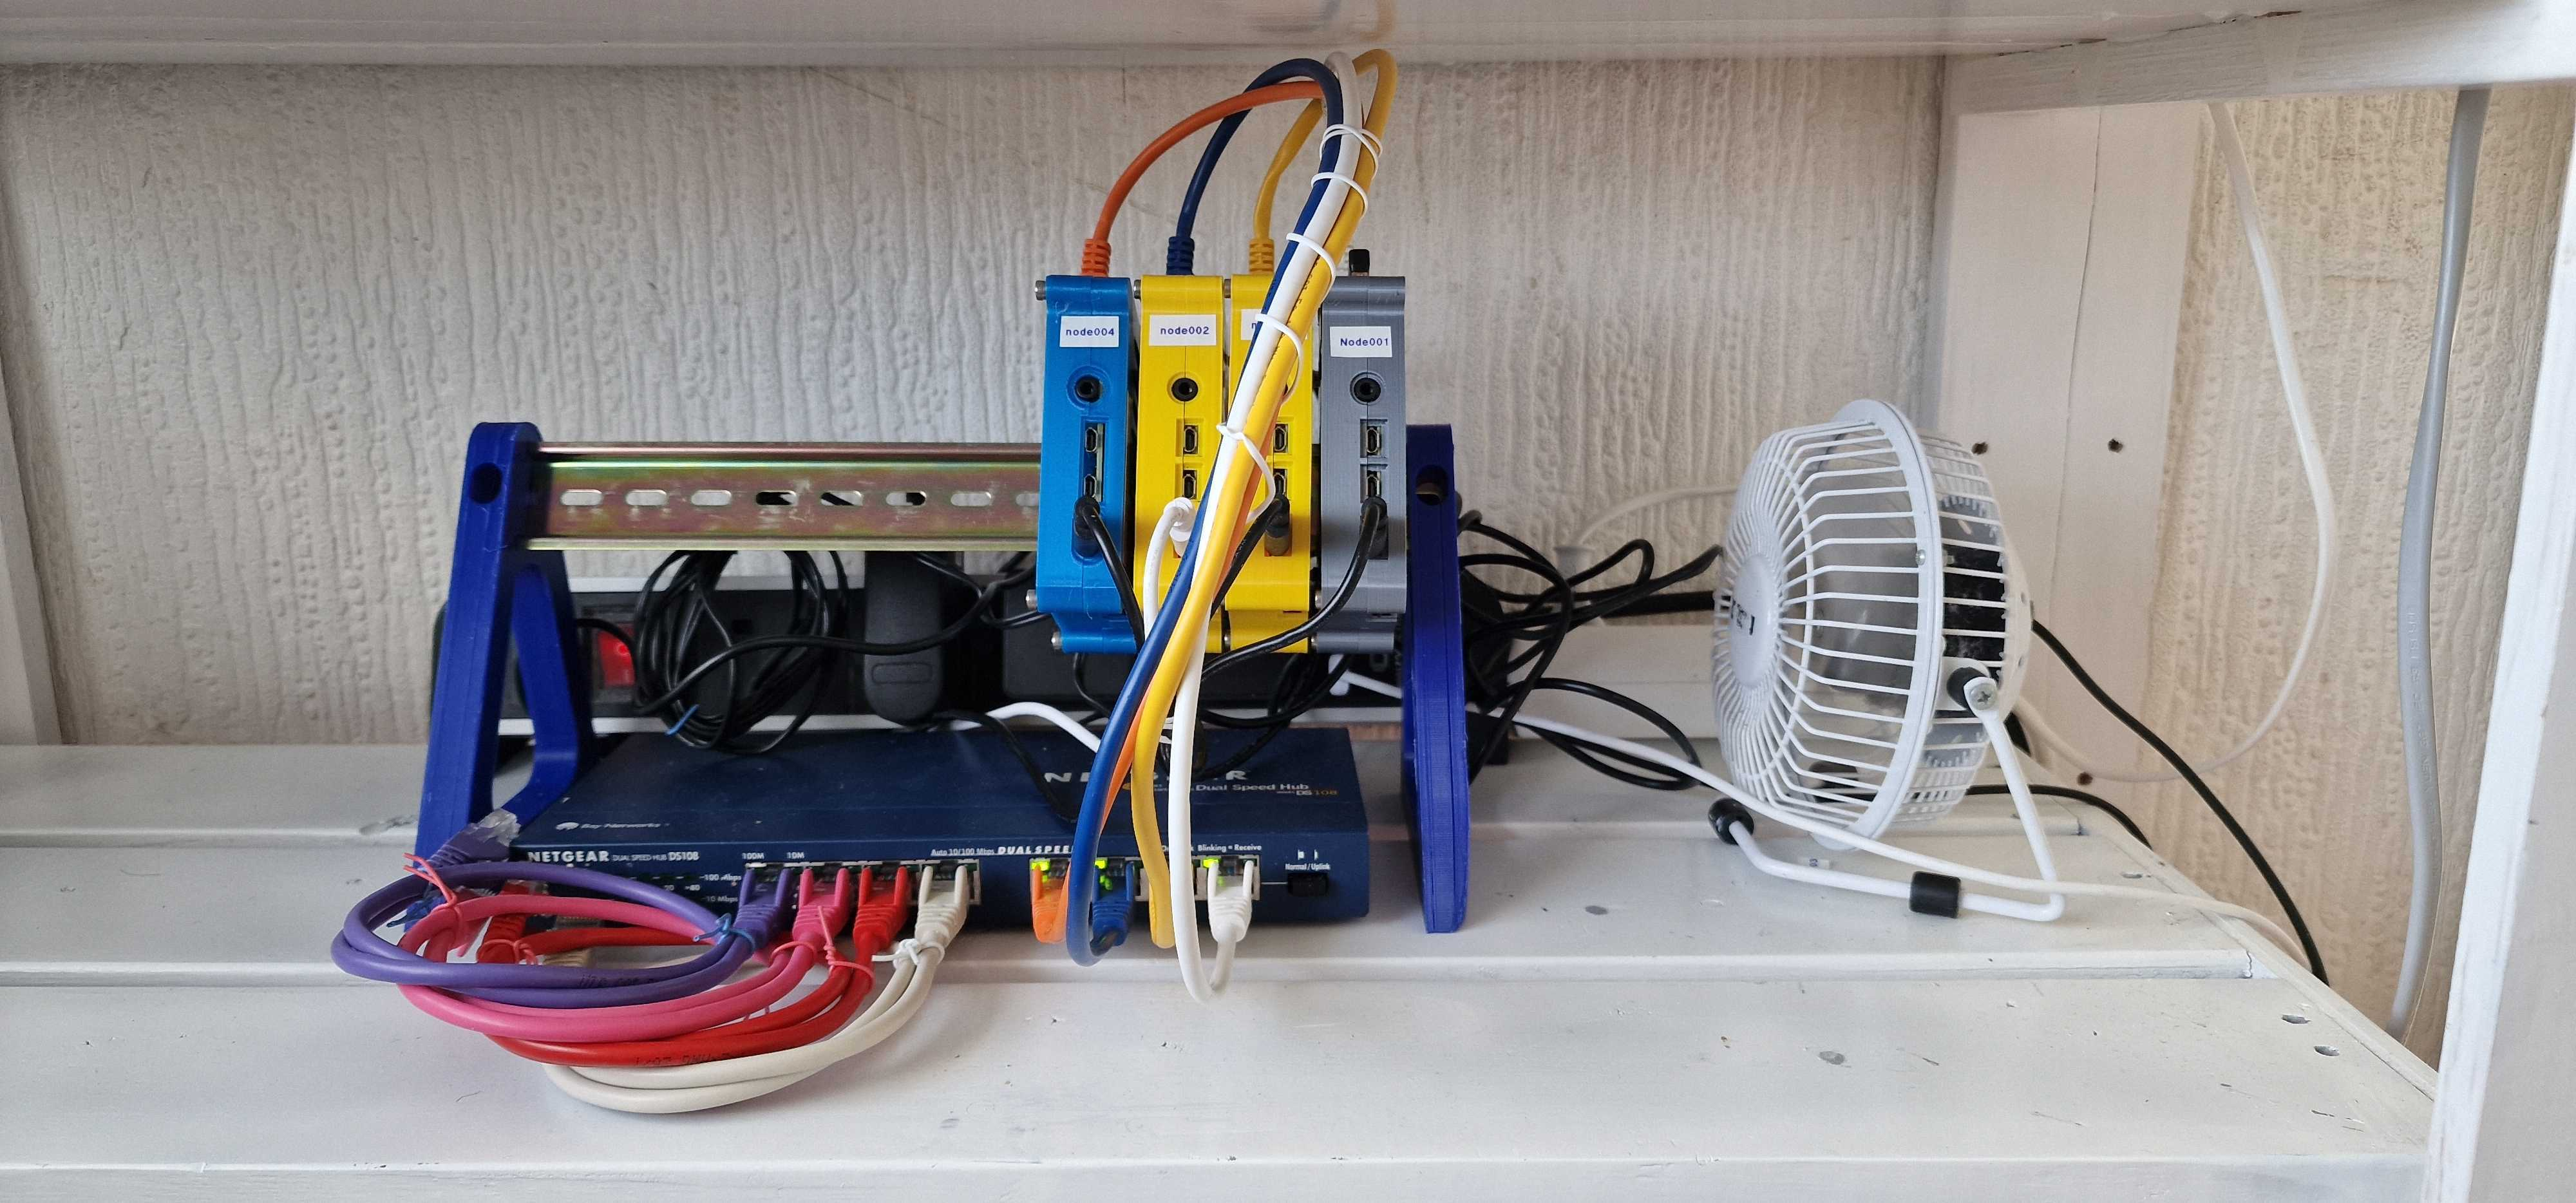
\includegraphics[width=0.9\columnwidth]{logos/mini-HPC-proto1.png}
							\caption{The prototype miniHPC built from RPi4s using RPi 4s that I had in the house. For the next iteration I bought Rock Pi 4C+}
						\end{center}
					\end{figure}
				\end{block}

				
				
				\begin{alertblock}{Pixie the Prototype}
					\begin{table}
						\parbox{.45\linewidth}{
						\centering
						\begin{tabular}{l c}
							\textbf{Item} & \textbf{Qty} \\
							\hline
							Raspberry Pi 4 & 5 \\
							Power supply & 5 \\
							8 port switch & 1 \\
							8 port strip plug & 1 \\
							Short Cat 6 10baseT & 8 \\
							Cooling fan & 1 \\
							DIN Rail & 1 \\
							3D printed rail stand & 2 \\
							3D printed DIN rail cases & 5 \\
							 & \\
						\end{tabular}
						\caption{BOM for Prototype miniHPC using Raspberry Pi 4s}			
						}
						\hfill
						\parbox{.45\linewidth}{
						\centering
						\begin{tabular}{l c}
							\textbf{Item} & \textbf{Qty} \\
							\hline
							RockPi 4C+ & 8 \\
							RockPi 4SE & 1 \\
							Power supply & 1 \\
							10 port switch & 1 \\
							4 port strip plug & 1 \\
							Short Cat 6 10baseT & 9 \\
							Dual Cooling fan & 1 \\
							DIN Rail & 1 \\
							3D printed rail stand & 2 \\
							3D printed DIN rail cases & 9 \\
						\end{tabular}
						\caption{BOM for RockPi 4C+ miniHPC}				
						}
					\end{table}
				\end{alertblock}	
			
			\parbox{.45\linewidth}{
			\centering
			\begin{block}{name1}
				stuf stuf stuf
			\end{block}
			}
			\hfill
			\parbox{.45\linewidth}{
			\centering
			\begin{block}{name2}
				stuff stuff stuff
			\end{block}
			}
						
			\end{column}			
			\separatorcolumn
		\end{columns}
	\end{frame}
	
\end{document}
